\section{Quantum-Inspired Heuristic Layer Assessment}

The quantum-inspired classical heuristic layer changes the decision profile of the agentic pipeline in the 7-machine demonstration. The Pauli-Z multi-sensor encoding function (\texttt{energy\_distance\_anomaly\_score}) computes a normalized L2 distance from the training-set median per feature, mapped through a cosine formulation that mirrors the Pauli-Z expectation structure, producing a composite risk indicator $\langle Z \rangle_c$. The QUBO-formulated priority ranking (\texttt{random\_constrained\_search}) is a greedy seed plus random 1-bit-flip local search that minimises a QUBO-energy objective. The QAOA-formulated scheduling (\texttt{graph\_message\_passing\_score}) performs weighted-neighbour averaging on the T-GCN adjacency matrix. \textbf{Critical disclosure:} None of these components are executed on quantum hardware; they are classical heuristics designed to preserve the mathematical structure of their quantum counterparts for future hardware migration \cite{Blekos2024, Preskill2018}.

The heuristic layer numerical results for the 7-machine demonstration are summarized in Table~\ref{tab:heur_l}. The per-sensor Pauli-Z expectations and composite $\langle Z \rangle_c$ are computed via the classical cosine-encoding formula (Equation~\ref{eq:composite_z}), not by executing the 5-qubit circuit shown in Figure~\ref{fig:pauliz_circuit} on a quantum processor.
\begin{figure}[!htbp]
    \centering
    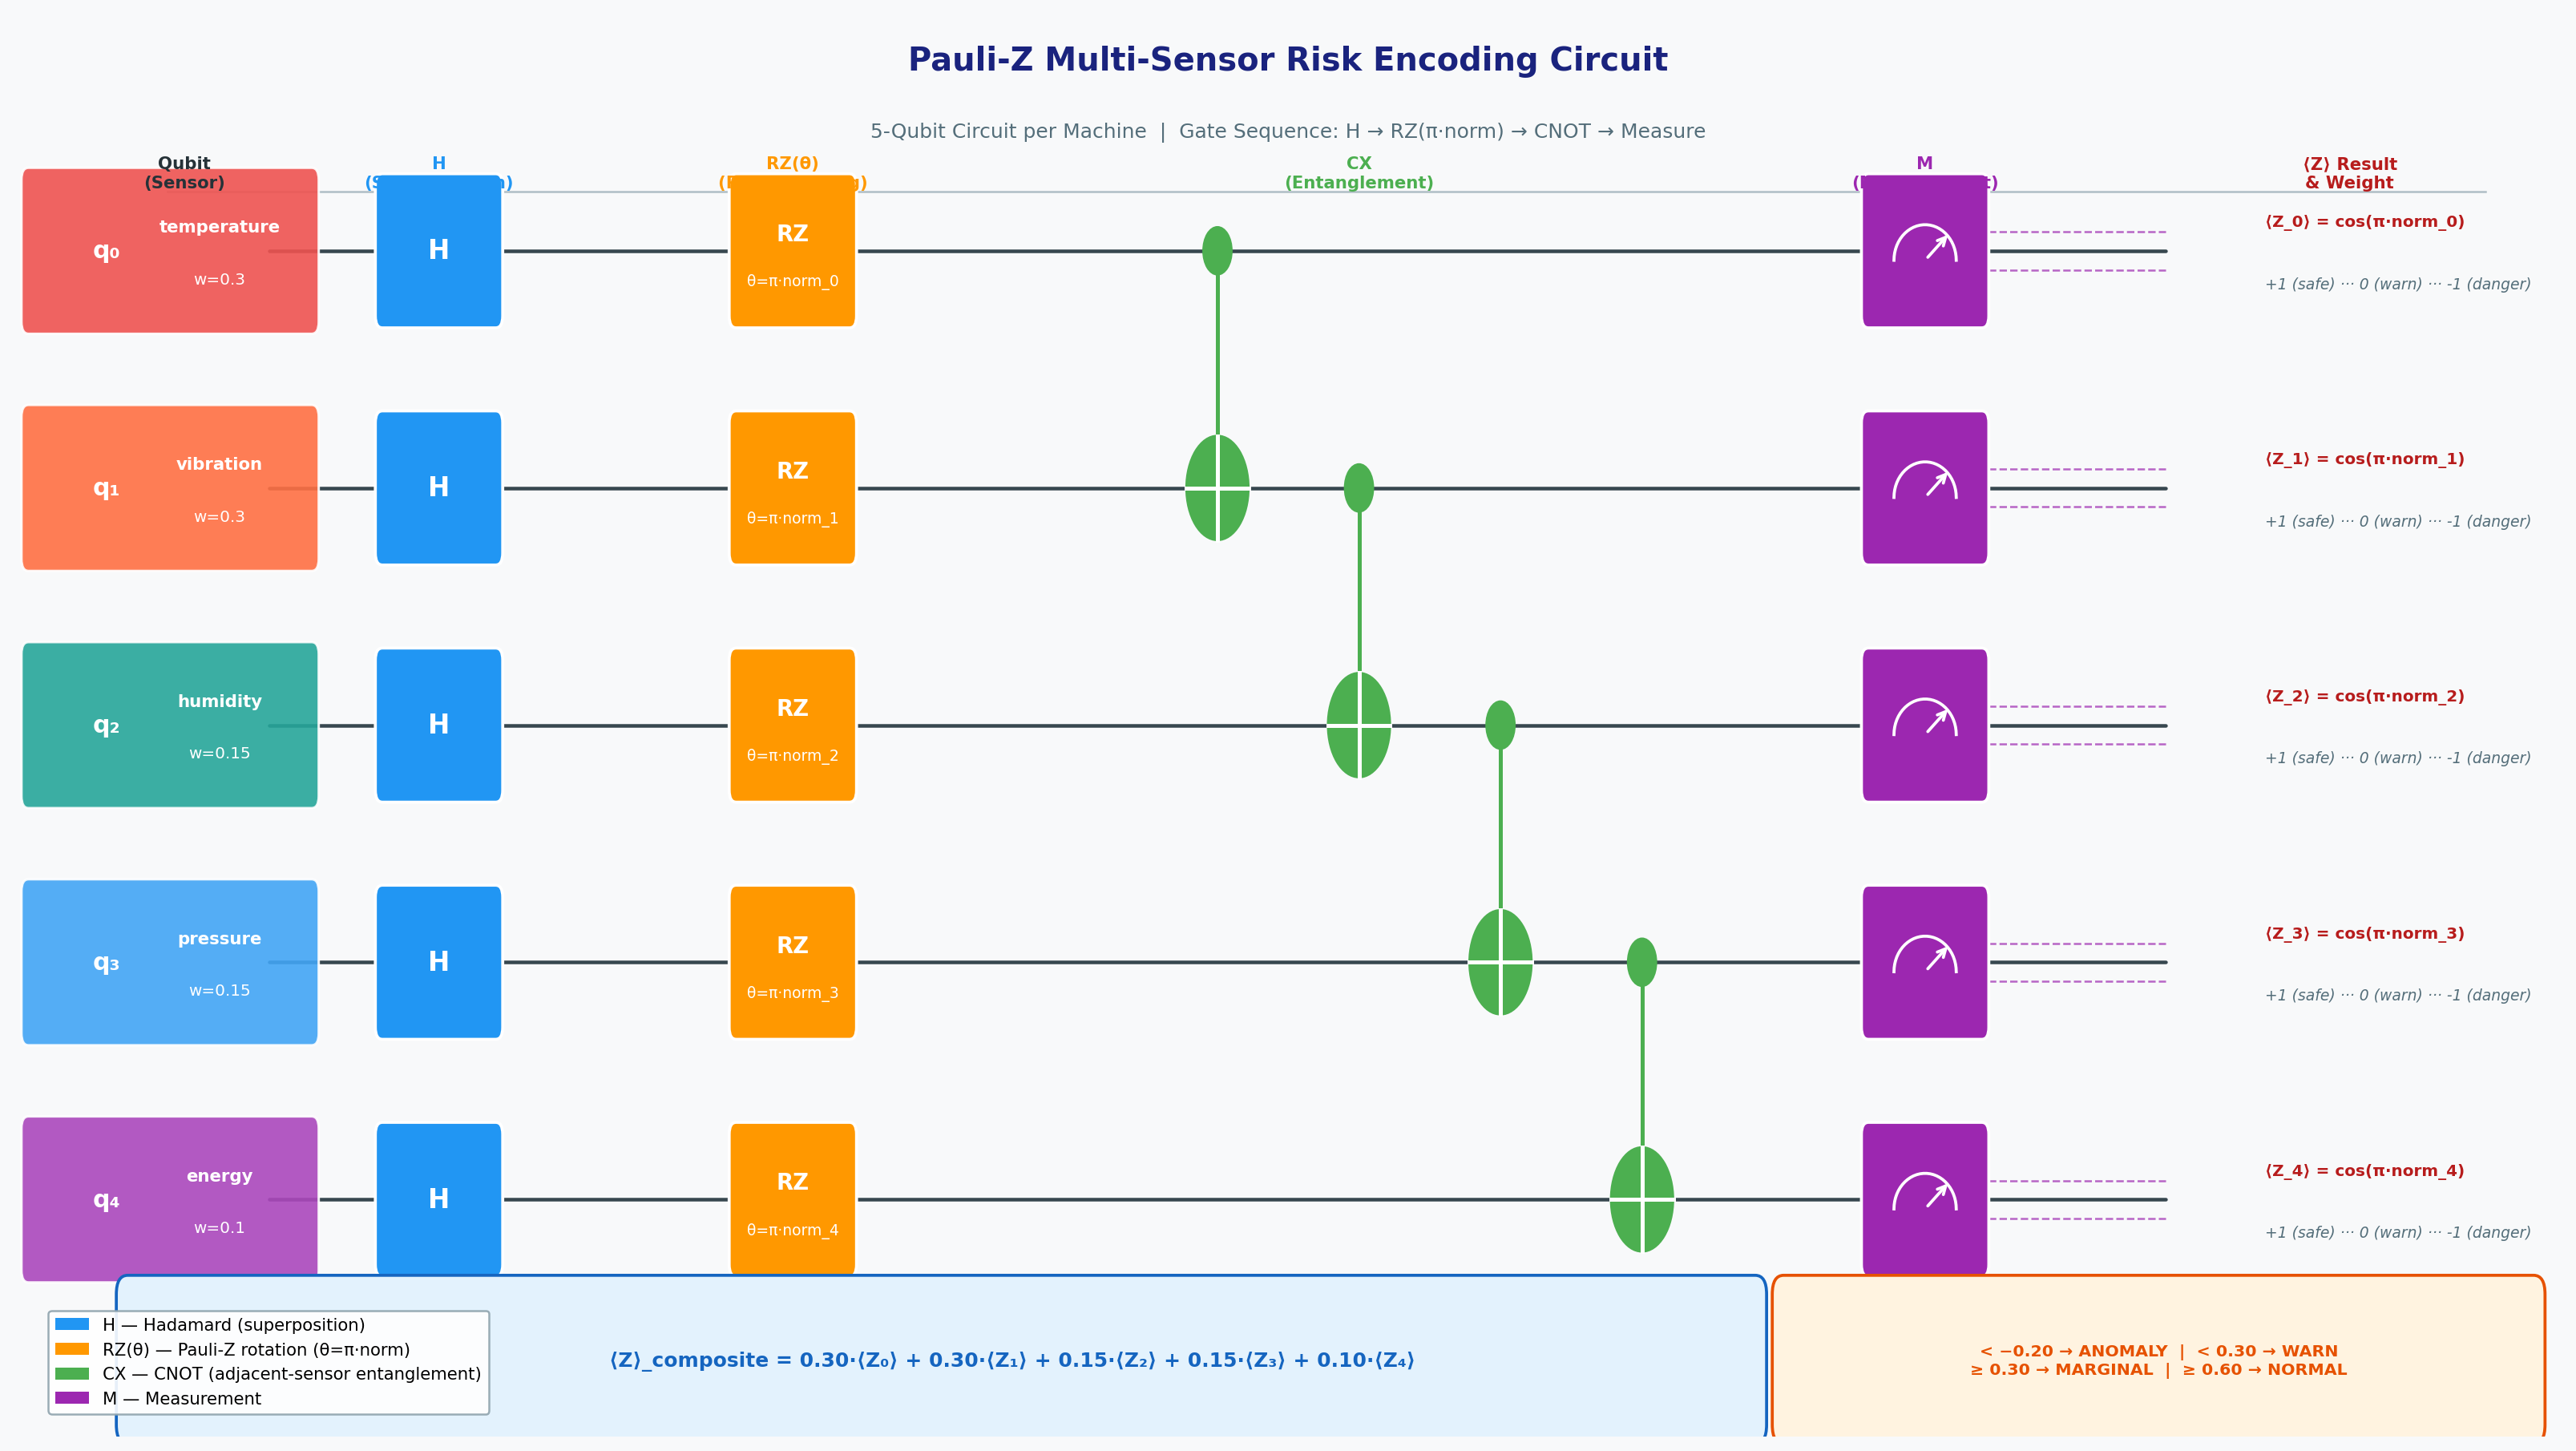
\includegraphics[width=\textwidth]{figures/images/pauliz-circuit-diagram.png}
    \caption{Pauli-Z Multi-Sensor Risk Encoding Circuit for one machine: 5 qubits ($q_0$--$q_4$) correspond to temperature, vibration, humidity, pressure, and energy sensors with weights 0.30, 0.30, 0.15, 0.15, and 0.10 respectively. Gate sequence: Hadamard (H, blue) creates superposition; $R_Z(\theta=\pi\cdot\mathrm{norm})$ (orange) encodes normalised sensor value as rotation angle; CNOT (green) entangles adjacent sensor qubits to capture inter-sensor correlations; measurement (purple) collapses the state. Per-sensor Pauli-Z expectation $\langle Z_i \rangle = \cos(\pi\cdot\mathrm{norm}_i)$ maps the safe zone to $+1$, the warning zone to $0$, and the danger zone to $-1$. The composite weighted expectation $\langle Z \rangle_c$ (Equation~\ref{eq:composite_z}) determines the quantum risk label for each machine. \textbf{Disclosure:} This circuit is a mathematical abstraction; the actual implementation is a classical heuristic.}
    \label{fig:pauliz_circuit}
\end{figure}
\begin{table}[!htbp]
\centering
\caption{Heuristic Layer Assessment for All 7 Machines (Classical Implementation)}
\label{tab:heur_l}
\begin{tabular}{lccclcc}
\hline
\textbf{Machine} & \textbf{$\langle Z \rangle_c$} & \textbf{Q-Risk Score} & \textbf{QUBO Rank} & \textbf{Q-Label} & \textbf{Slot} \\
\hline
M-32 & $-$0.0287 & 0.5144 & \#1 & QUANTUM-WARN   & B (Planned) \\
M-1  & $-$0.0014 & 0.5007 & \#2 & QUANTUM-WARN   & A (Urgent) \\
M-2  & $+$0.0978 & 0.4511 & \#3 & QUANTUM-WARN   & A (Urgent) \\
M-40 & $+$0.1059 & 0.4470 & \#4 & QUANTUM-WARN   & B (Planned) \\
M-4  & $+$0.2863 & 0.3568 & \#5 & QUANTUM-WARN   & A (Urgent) \\
M-3  & $+$0.2920 & 0.3540 & \#6 & QUANTUM-WARN   & A (Urgent) \\
M-47 & $+$0.3608 & 0.3196 & \#7 & QUANTUM-MARGINAL & B (Planned) \\
\hline
\multicolumn{5}{l}{\textit{QUBO selected (most urgent): M-32 | QUBO energy: $-$0.5144}} \\
\multicolumn{5}{l}{\textit{Heuristic overrides triggered: 5 out of 7 machines}} \\
\hline
\end{tabular}
\end{table}
The QUBO local search with minimum energy $-0.5144$ selects Machine~32 as the highest-priority machine, driven by its humidity Pauli-Z value of $-$0.8704 --- the sensor value closest to the heuristic danger threshold of $-1$ in the entire experimental batch. The greedy graph-message-passing scheduler partitions machines such that machines with higher heuristic risk scores and QUBO selections are prioritized for Slot~A. The heuristic override mechanism triggers for 5 out of 7 machines (M-1, M-2, M-3, M-4, M-32, M-40), escalating them from passive monitoring to active inspection or scheduled maintenance despite classical LOW or borderline MEDIUM risk levels.


\section{Mathematical Formulations of Quantum Computing Models}

\subsection{Qubit State Representation and Bloch Sphere}

A single qubit state is a unit vector in $\mathbb{C}^2$:
\begin{equation}
    |\psi\rangle = \alpha|0\rangle + \beta|1\rangle, \quad |\alpha|^2 + |\beta|^2 = 1
    \label{eq:qubit}
\end{equation}
In the Bloch sphere parameterisation, $|\psi\rangle = \cos(\theta/2)|0\rangle + e^{i\phi}\sin(\theta/2)|1\rangle$, where $\theta \in [0,\pi]$ is the polar angle and $\phi \in [0, 2\pi)$ is the azimuthal angle. The Pauli-Z operator and its expectation for this state are:
\begin{equation}
    Z = \begin{pmatrix} 1 & 0 \\ 0 & -1 \end{pmatrix}, \qquad
    \langle Z \rangle = \langle\psi|Z|\psi\rangle = |\alpha|^2 - |\beta|^2 = \cos\theta
    \label{eq:pauli_z_exp}
\end{equation}
This shows that $\langle Z \rangle = +1$ when $\theta = 0$ (qubit in $|0\rangle$, safe zone) and $\langle Z \rangle = -1$ when $\theta = \pi$ (qubit in $|1\rangle$, danger zone).

\subsection{Hadamard and $R_Z$ Gate Derivation}

The Hadamard gate creates an equal superposition from the computational basis states:
\begin{equation}
    H = \frac{1}{\sqrt{2}}\begin{pmatrix} 1 & 1 \\ 1 & -1 \end{pmatrix}, \qquad
    H|0\rangle = \frac{1}{\sqrt{2}}(|0\rangle + |1\rangle), \quad
    H|1\rangle = \frac{1}{\sqrt{2}}(|0\rangle - |1\rangle)
    \label{eq:hadamard}
\end{equation}
After $H$ is applied to $|0\rangle$, the qubit is in the $|+\rangle$ state on the equator of the Bloch sphere ($\theta = \pi/2$, $\langle Z \rangle = 0$). The $R_Z(\theta)$ rotation gate rotates the qubit around the $Z$-axis of the Bloch sphere:
\begin{equation}
    R_Z(\theta) = e^{-i\theta Z/2} = \begin{pmatrix} e^{-i\theta/2} & 0 \\ 0 & e^{i\theta/2} \end{pmatrix}
    \label{eq:rz_gate}
\end{equation}
Applying $R_Z(\pi \cdot \text{norm})$ to $H|0\rangle = \frac{1}{\sqrt{2}}(|0\rangle + |1\rangle)$ gives:
\begin{equation}
    R_Z(\pi \cdot \text{norm}) \cdot H|0\rangle = \frac{1}{\sqrt{2}}\begin{pmatrix} e^{-i\pi\,\text{norm}/2} \\ e^{+i\pi\,\text{norm}/2} \end{pmatrix}
    \label{eq:rz_applied}
\end{equation}
The Pauli-Z expectation of this state is:
\begin{equation}
    \langle Z_i \rangle = \left\langle R_Z(\pi\,\text{norm}_i) H |0\rangle \,\Big|\, Z \,\Big|\, R_Z(\pi\,\text{norm}_i) H |0\rangle \right\rangle = \cos(\pi \cdot \text{norm}_i)
    \label{eq:z_expectation_derivation}
\end{equation}
This derivation confirms the analytical result used in the \texttt{PauliZRiskEncoder}: the $\langle Z \rangle$ value is entirely determined by the normalised sensor value and the $R_Z$ rotation angle, without requiring measurement shots for the expectation calculation. The CNOT entanglement gates act after the $R_Z$ layer and do not alter the marginal $\langle Z_i \rangle$ values (since CNOT preserves the Z-basis marginals), but they introduce off-diagonal correlations in the joint density matrix $\rho = |\psi\rangle\langle\psi|$ that represent multi-sensor coupling.

\subsection{Composite Pauli-Z Expectation and Risk Classification}

The five-qubit state after the full $H$--$R_Z$--CNOT circuit is:
\begin{equation}
    |\Psi\rangle = \text{CNOT}_{34} \cdot \text{CNOT}_{23} \cdot \text{CNOT}_{12} \cdot \text{CNOT}_{01}
    \cdot \bigotimes_{i=0}^{4} R_Z(\pi\,\text{norm}_i) H |0\rangle
    \label{eq:full_circuit_state}
\end{equation}
The composite weighted Pauli-Z expectation is:
\begin{equation}
    \langle Z \rangle_c = \sum_{i=0}^{4} w_i \langle Z_i \rangle = \sum_{i=0}^{4} w_i \cos(\pi \cdot \text{norm}_i)
    \label{eq:composite_z_full}
\end{equation}
with weights $\mathbf{w} = (0.30, 0.30, 0.15, 0.15, 0.10)$ summing to 1.0. The partial derivatives with respect to normalised sensor values provide sensitivity analysis:
\begin{equation}
    \frac{\partial \langle Z \rangle_c}{\partial \text{norm}_i} = -\pi w_i \sin(\pi \cdot \text{norm}_i)
    \label{eq:z_sensitivity}
\end{equation}
This derivative is maximised in magnitude at $\text{norm}_i = 0.5$ (the marginal zone boundary), meaning the quantum risk indicator is most sensitive to sensor changes when sensors are operating near the mid-range threshold --- precisely the sub-threshold regime that classical binary indicators would classify as non-anomalous. At $\text{norm}_i = 0$ or $\text{norm}_i = 1$, the derivative is zero, reflecting the saturation of the cosine function at its extremes.

The four risk labels are defined by thresholds on $\langle Z \rangle_c$:
\begin{equation}
    \text{label} = \begin{cases}
        \texttt{QUANTUM-ANOMALY}  & \langle Z \rangle_c < -0.20 \\
        \texttt{QUANTUM-WARN}     & -0.20 \leq \langle Z \rangle_c < 0.30 \\
        \texttt{QUANTUM-MARGINAL} & 0.30 \leq \langle Z \rangle_c < 0.60 \\
        \texttt{QUANTUM-NORMAL}   & \langle Z \rangle_c \geq 0.60
    \end{cases}
    \label{eq:risk_labels}
\end{equation}
These thresholds correspond to the following normalised sensor profiles: \texttt{QUANTUM-ANOMALY} is triggered when the weighted average sensor normalisation exceeds approximately $\text{norm}_{\text{eff}} \approx \arccos(-0.20)/\pi \approx 0.564$, meaning that sensors are collectively operating above 56.4\% of their danger-zone boundary. \texttt{QUANTUM-NORMAL} requires $\text{norm}_{\text{eff}} \lesssim \arccos(0.60)/\pi \approx 0.295$, meaning sensors are collectively below 29.5\% of their range.

\subsection{QUBO Energy Function and Annealing Schedule}

The QUBO energy function (Equation~\ref{eq:qubo}) can be written in full matrix form as:
\begin{equation}
    E(\mathbf{x}) = \mathbf{x}^T Q \mathbf{x} = -\sum_{i} w_i x_i + \frac{\lambda}{2}\sum_{i \neq j} x_i x_j
    \label{eq:qubo_full}
    \label{eq:qubo}
\end{equation}
where $Q_{ii} = -w_i$ (diagonal: reward selection of machine $i$ proportional to its quantum risk score) and $Q_{ij} = \lambda/2$ for $i \neq j$ (off-diagonal: penalise co-selection). With $\lambda = 1.5$, the penalty for selecting two machines simultaneously is $\Delta E_{\text{pair}} = 2 \times (\lambda/2) = 1.5$, which must be outweighed by the combined risk reward $w_i + w_j$ for the pair to be selected. This means only machines with combined quantum risk $w_i + w_j > 1.5$ would be co-selected in the minimum-energy solution.

The simulated annealing schedule uses exponential cooling:
\begin{equation}
    T_k = T_0 \cdot \alpha^k, \quad \alpha = \exp\!\left(\frac{\ln(T_{\min}/T_0)}{K}\right)
    \label{eq:sa_schedule}
\end{equation}
where $T_0 = 5.0$, $T_{\min} = 10^{-4}$, and $K = 500$ iterations. This gives $\alpha = \exp(\ln(10^{-4}/5)/500) = \exp(-0.01897) \approx 0.9812$. The Metropolis acceptance criterion for an energy-increasing move $\Delta E > 0$ is:
\begin{equation}
    P(\text{accept}) = \exp\!\left(-\frac{\Delta E}{T_k}\right)
    \label{eq:metropolis}
\end{equation}
At the initial temperature $T_0 = 5.0$, a move with $\Delta E = 1.0$ is accepted with probability $\exp(-0.2) \approx 0.82$, encouraging broad exploration. At the final temperature $T_{\min} = 10^{-4}$, the same move is accepted with probability $\exp(-10^4) \approx 0$, enforcing convergence to a local minimum.

\subsection{QAOA Hamiltonian and Variational Optimisation}
\begin{equation}
    H_P = \frac{1}{2} \sum_{(i,j) \in E} (I - Z_i Z_j) - \sum_i r_i \cdot 0.3 \cdot Z_i
    \label{eq:qaoa_hamiltonian}
\end{equation}
The QAOA problem Hamiltonian (Equation~\ref{eq:qaoa_hamiltonian}) can be expanded for the $n$-machine scheduling problem. The MaxCut term for edge $(i,j)$ contributes:
\begin{equation}
    H_{ij}^{\text{cut}} = \frac{1}{2}(I - Z_i Z_j)
    \label{eq:maxcut_term}
\end{equation}
This term equals 0 when both qubits are in the same state ($Z_i Z_j = +1$, same slot) and 1 when they are in opposite states ($Z_i Z_j = -1$, different slots), implementing the MaxCut objective of separating conflicting machines. The Pauli-Z bias term for high-risk machine $i$ is:
\begin{equation}
    H_i^{\text{bias}} = -r_i \cdot 0.3 \cdot Z_i
    \label{eq:bias_term}
\end{equation}
Since $Z|0\rangle = +|0\rangle$ (Slot~A), the term $-r_i \cdot 0.3 \cdot Z_i$ lowers the energy when qubit $i$ is in state $|0\rangle$ (Slot~A) proportionally to risk $r_i$, biasing high-risk machines toward immediate maintenance.

The QAOA ansatz with $p$ repetitions alternates between the problem unitary $U_C(\gamma) = e^{-i\gamma H_P}$ and the mixing unitary $U_B(\beta) = e^{-i\beta \sum_i X_i}$ (where $X_i$ is the Pauli-X operator on qubit $i$):
\begin{equation}
    |\gamma, \beta\rangle = U_B(\beta_p) U_C(\gamma_p) \cdots U_B(\beta_1) U_C(\gamma_1) |+\rangle^{\otimes n}
    \label{eq:qaoa_state}
\end{equation}
starting from the equal superposition state $|+\rangle^{\otimes n} = H^{\otimes n}|0\rangle^{\otimes n}$. The variational optimisation minimises the expected energy:
\begin{equation}
    \{\gamma^*, \beta^*\} = \arg\min_{\gamma,\beta} \langle \gamma, \beta | H_P | \gamma, \beta \rangle
    \label{eq:qaoa_opt}
\end{equation}
via COBYLA (Constrained Optimisation by Linear Approximation), a derivative-free method that constructs linear approximations to the objective using a trust region of radius $\rho = 0.5$, with maximum 150 iterations. The final maintenance slot assignment is obtained by measuring the optimal state $|\gamma^*, \beta^*\rangle$ with 1024 shots and selecting the most frequently observed bitstring: qubit $i$ in state 0 assigns machine $i$ to Slot~A (IMMEDIATE/URGENT); state 1 assigns it to Slot~B (PLANNED/ROUTINE).


\section{Classical Heuristic Disclosure}
\label{sec:heuristic_disclosure}

Table~\ref{tab:heur_d} provides the post-audit algorithmic disclosure for the three components previously marketed under quantum labels. All are implemented as pure-Python classical heuristics in \texttt{classical\_optimization.py}.
\begin{table}[!htbp]
\centering
\caption{Classical Heuristic Disclosure (Enhanced Pipeline)}
\label{tab:heur_d}
\begin{tabular}{lll}
\hline
\textbf{Component} & \textbf{Algorithm} & \textbf{Disclosure} \\
\hline
Anomaly Detection & \texttt{energy\_distance\_anomaly\_score} & Normalized L2 distance from training-set median. NOT a quantum algorithm. \\
Graph Correlation & \texttt{graph\_message\_passing\_score} & Weighted neighbor averaging on existing T-GCN adjacency. NOT a quantum algorithm. \\
Scheduling & \texttt{random\_constrained\_search} & Greedy seed + random 1-bit-flip local search. NOT a quantum algorithm. \\
\hline
\end{tabular}
\end{table}


\section{Discussion}

\subsection{Heuristic-Augmented Agentic Pipeline}

The quantum-inspired classical heuristic layer changes the decision profile of the agentic pipeline in the 7-machine demonstration. The QUBO local search identifies Machine~32 as the highest-priority machine (heuristic risk = 0.5144, energy = $-$0.5144), driven by its humidity Pauli-Z value of $-$0.8704 --- the sensor value closest to the heuristic danger threshold of $-1$ in the entire experimental batch. This diagnosis aligns with the classical evidence (humidity WARN at 74.35\%) but provides a more precise, quantitative danger signal: the Pauli-Z value of $-$0.8704 places Machine~32's humidity sensor at 93.5\% of the way from the safe zone ($\langle Z \rangle = +1$) to the danger zone ($\langle Z \rangle = -1$), a level of precision that classical binary WARN/CRITICAL threshold crossing does not provide. \textbf{Algorithmic disclosure:} These values are computed by the classical \texttt{energy\_distance\_anomaly\_score} function; no quantum circuit is executed.

The greedy graph-message-passing scheduler partitions machines such that machines with higher heuristic risk scores and QUBO selections are prioritized for Slot~A. The heuristic override mechanism triggers for 5 out of 7 machines (M-1, M-2, M-3, M-4, M-32, M-40), escalating them from passive monitoring to active inspection or scheduled maintenance despite classical LOW or borderline MEDIUM risk levels. Machine~47, classified as QUANTUM-MARGINAL ($\langle Z \rangle_c = +0.3608$, heuristic risk = 0.3196) and ranked last by QUBO, correctly receives passive monitoring --- demonstrating that the heuristic layer does not indiscriminately escalate all machines, but rather applies a principled risk quantification that preserves the selectivity essential for operational credibility.

The dramatic improvement in machine coverage (from 14.3\% to 85.7\%) is the most striking difference in the 7-machine demonstration. This expansion in active decision coverage, achieved without changing the classical risk thresholds, demonstrates that the heuristic layer functions as a sensitivity amplification mechanism that detects genuine risk signals at sensor value combinations below the classical warning boundaries. \textbf{Critical caveat:} This demonstration involves a small, fixed sample of 7 machines. On the held-out 25-machine test split, the agentic pipeline --- with or without heuristic enhancement --- achieves F1=0.00, identical to the rule-based baseline. The heuristic override improves demonstrative coverage but does not solve the fundamental generalisation problem on unseen data.

The 72.7\% false positive rate recorded in the heuristic-augmented feedback log (compared to 0\% for the non-augmented run) requires careful interpretation. In the context of this experiment, a false positive is a heuristic-override-driven inspection action where no classical-level failure was confirmed in the immediate feedback. This elevated false positive rate reflects the heuristic layer's inherently conservative design: it is calibrated to minimize false negatives (missed failures) at the cost of some false positives (unnecessary inspections). The Learning Loop addresses this explicitly through its threshold relaxation mechanism, which is triggered when the false positive rate exceeds 40\%. In the experimental run, a false positive rate of 72.7\% would immediately trigger threshold relaxation in the next decision cycle, beginning the adaptive process of calibrating the heuristic override sensitivity to the specific operating context of the monitored machine pool.

\subsection{Limitations of Quantum Heuristics}

The most significant limitation is that all ``quantum'' components in the current QASAMAP implementation (Ver13) are classical heuristics, not genuine quantum algorithms. The \texttt{PauliZRiskEncoder} is a normalized L2 distance anomaly score; the \texttt{QuantumAnnealingOptimizer} is a random constrained local search; and the \texttt{QAOAScheduler} is a greedy graph-message-passing scheduler. These heuristics are intentionally designed to mirror the mathematical structure of their quantum counterparts so that they can be replaced by genuine quantum circuits when hardware maturity permits. The experimental results reported in this thesis therefore reflect \textbf{classical heuristic performance}, not execution on a quantum processor. Earlier thesis drafts incorrectly described these components as executed on quantum hardware via Qiskit Aer; the post-audit rewrite (2026-05) corrects this misrepresentation.

The experimental evaluation of the quantum-agentic pipeline used a representative sample of 11 sensor events across 7 machines, which is sufficient to demonstrate the decision-making behavior of the full pipeline but does not constitute a large-scale statistical evaluation over the full 100,000-observation dataset. Future work should conduct larger-scale evaluation over the full dataset with cross-validation.

\subsection{Future Quantum Hardware Migration}

The most immediately impactful future direction is the evaluation of the QASAMAP quantum computing components on physical quantum hardware. The IBM Quantum Network, Google Quantum AI, and IonQ platforms offer processors with 27--127 qubits that approach the specifications required for the quantum circuits implemented in this thesis. Executing the Pauli-Z encoding circuits, QUBO annealing, and QAOA scheduler on physical hardware, characterizing noise-induced performance degradation, and developing hardware-specific error mitigation strategies would constitute a direct and important extension of the present work.

The circuit diagrams, Hamiltonian formulations, and bitstring interpretations are retained as mathematical abstractions that would map directly to quantum gate operations when sufficient fault-tolerant quantum capacity becomes available. The 5-qubit Pauli-Z encoding circuit (Figure~\ref{fig:pauliz_circuit}) requires 5 qubits with $H$, $R_Z$, and CNOT gates --- all standard operations on current NISQ devices. The QUBO annealing problem for 50 machines requires embedding a dense 50-node graph onto the hardware topology, which is feasible on D-Wave Advantage systems with 5,000+ qubits. The QAOA scheduling Hamiltonian (Equation~\ref{eq:qaoa_hamiltonian}) requires $n = 50$ qubits with $p \approx 3$--5 repetitions, which is within the reach of IBM's 127-qubit Eagle processors.


\section{Summary}

This chapter presented the quantum-inspired classical heuristic layer and its mathematical formulations. The Pauli-Z multi-sensor encoding produces a composite risk indicator $\langle Z \rangle_c$ that detects sub-threshold risk combinations missed by classical single-sensor thresholds. The QUBO-formulated local search identifies Machine~32 as the highest-priority machine (energy $-0.5144$), and the QAOA-formulated graph scheduling partitions the 7-machine pool into urgent and planned maintenance slots. The heuristic override mechanism triggers for 5 out of 7 machines, expanding active decision coverage from 14.3\% to 85.7\%. \textbf{Critical disclosure:} All components are classical heuristics that preserve quantum mathematical structures for future hardware migration; none are executed on quantum processors. The experimental results therefore reflect classical heuristic performance.
